\chapter{Исследование параметров РТГС на основе $Al_{x}Ga_{1-x}As$}
\section{Исследование параметров ямы}
Энергетический спектр в бесконечно глубокой потенциальной яме:
\begin{gather}
	\label{eq:En}
	E_{n} = \frac{\pi^{2}\hbar^{2}n^{2}}{2mL^{2}};\\
	\Delta E_{n} = E_{n+1} - E_{n} = \frac{\pi^{2}\hbar^{2}}{2mL^{2}}(2n + 1);\\
	\label{eq:dEn1}
	\Delta E_{1} = \min(\Delta E_{n}) = \frac{3\pi^{2}\hbar^{2}}{2mL^{2}},
\end{gather}
\begin{conditions}
	$E_{n}$ & энергия $n$-ого связного состояния;\\
	$\hbar$ & постоянная Дирака;\\
	$n$ & номер ($1,\,,2,\dots$) связного состояния;\\
	$L$ & ширина ямы.
\end{conditions}

Из зависимостей~\ref{eq:En},~\ref{eq:dEn1}  видно, что с увеличением ширины ямы, энергия основного состояния уменьшается ($n = 1$), так же, как и минимальное расстояние, между энергетическими уровнями. Условие размерного квантования для потенциальной ямы:
\begin{equation}
	\Delta E_{1} \gg 3k_{B}T.
\end{equation}

В случаи ямы с конечной высотой, энергия основного и остальных состояний понижается, при этом минимальная высота барьера ограничивает состояние с максимальной энергией. В потенциальной яме конечной высоты всегда будет хотя бы одно связное состояние.

\subsection{Исследование глубины ямы}
Варьирую процентное содержание $Al$ в $Al_{x}Ga_{1-x}As$, можно изменять высоту барьеров и глубину ямы соответственно. Рассмотрим вольт-амперную характеристику и прозрачность резонансно-туннельной структуры.

Так как в ходе деградации ГС высота барьеров будет уменьшаться, так как атомы $Al$ будут диффундировать в структуру из барьеров, рассмотрим РГТС (рис.~\ref{img:rtgs}) с высотой потенциальных барьеров:
\begin{enumerate}
	\item $1.0 eV$;
	\item $0.7 eV$;
	\item $0.5 eV$;
	\item $0.3 eV$.
\end{enumerate}

\subsubsection{Прозрачность РТГС}
\begin{figure}[h]
	\centering
	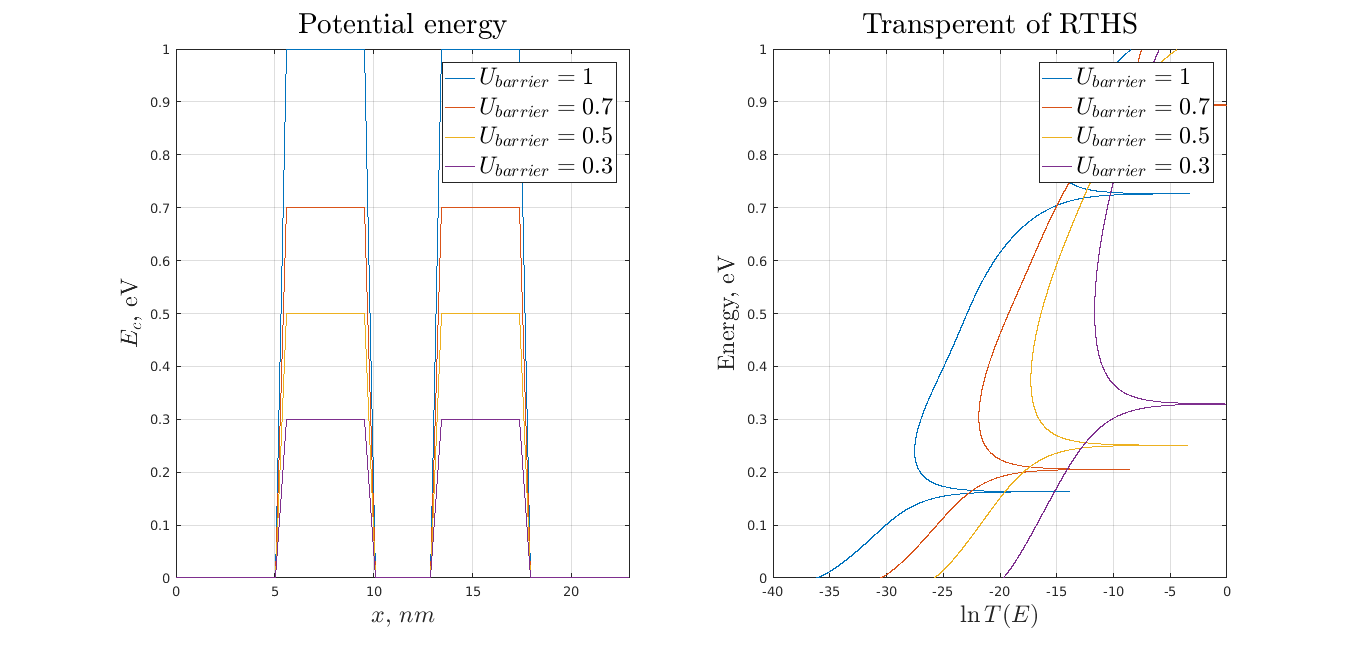
\includegraphics[width=\linewidth]{qwt.png}
	\caption{Прозрачность РТГС при различных высотах потенциального барьера}
	\label{fig:qwt}
\end{figure}

Как видно из рис.~\ref{fig:qwt} уменьшение высоты барьеров ведет к повышению резонансного уровня и увеличению коэффициента прозрачности исследуемой РТГС. 

\subsubsection{ВАХ РТГС}
\begin{figure}[h]
	\centering
	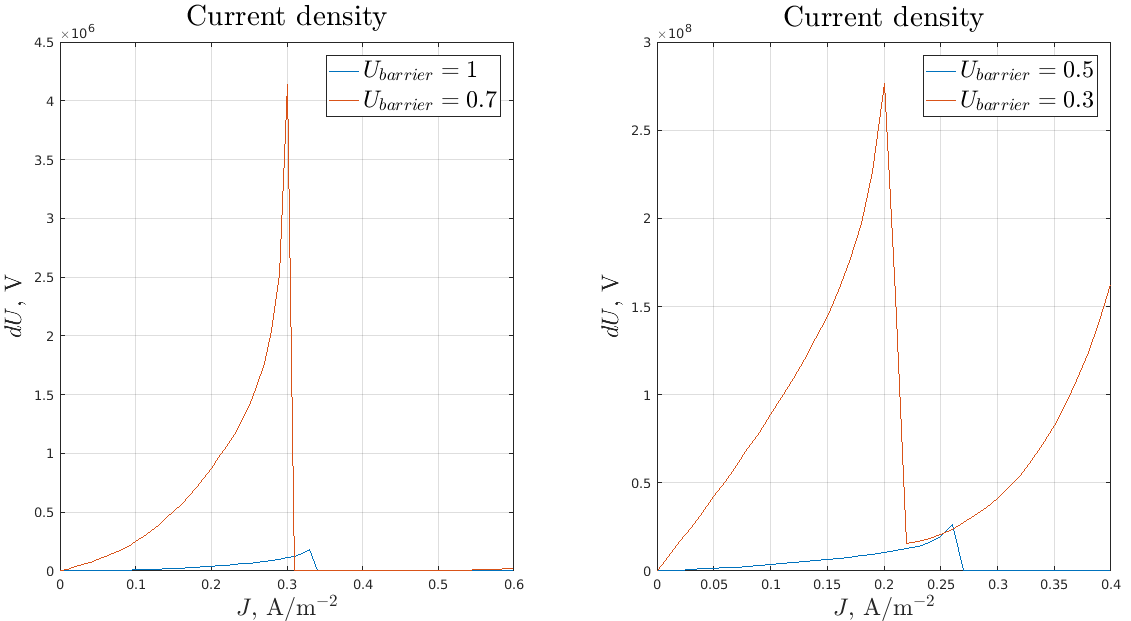
\includegraphics[width=\linewidth]{qwj.png}
	\caption{Плотность тока через РТГС при различных высотах потенциального барьера}
	\label{fig:qwj}
\end{figure}

Поднятие резонансного уровня на рис.~\ref{fig:qwt} увеличило напряжение, при котором достигается пиковое значение тока. Увеличение коэффициента прозрачности повысило пиковое значение тока на один порядок с изменением высоты барьеров на $0.2$эВ (рис.~\ref{fig:qwj}).

\subsection{Исследование ширины ямы}
Уменьшая или увеличивая количество монослоев, мы варьируем ширину ямы в РТГС. Минимальная разница между соседними уровнями и энергия этих уровней уменьшаются с увеличением ширины ямы (см. (\ref{eq:En}) -- (\ref{eq:dEn1})).

Для исследования влияния ширины ямы, рассмотрим следующий ряд ширины ям:
\begin{enumerate}
	\item $10$ монослоев;
	\item $7$ монослоев;
	\item $5$ монослоев;
	\item $3$ монослоев.
\end{enumerate}

\subsubsection{Прозрачность РТГС}
\begin{figure}[h!]
	\centering
	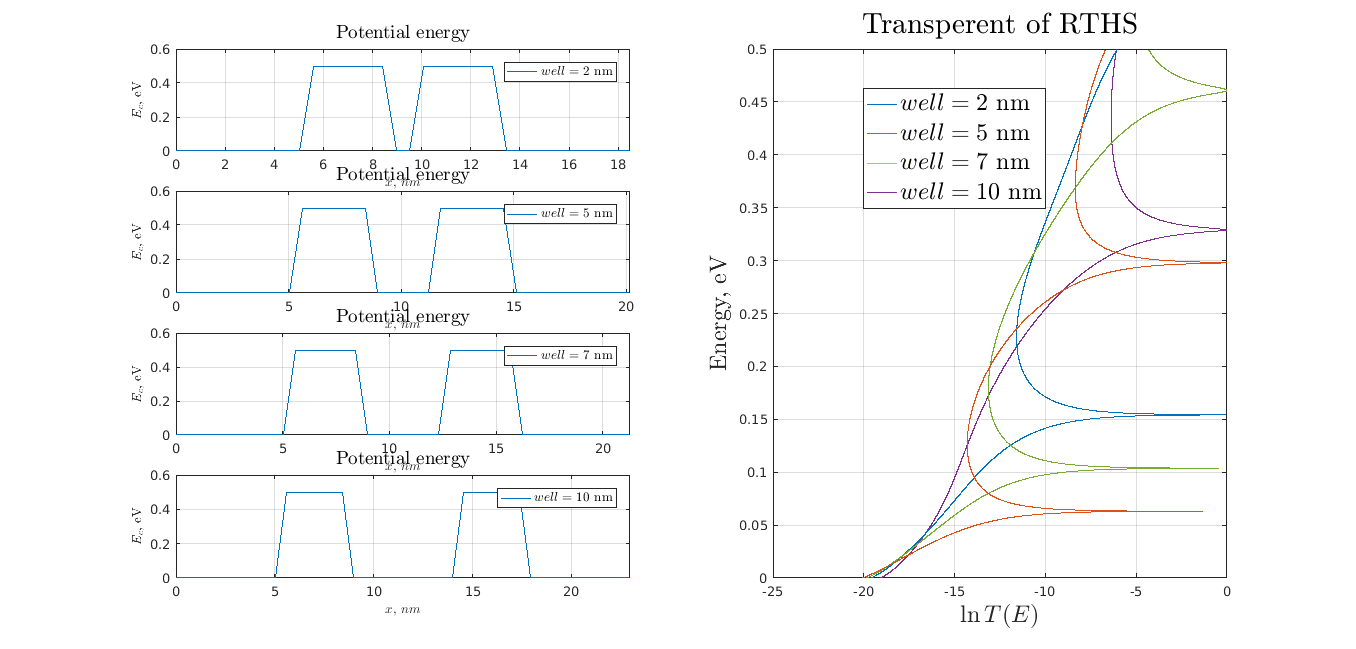
\includegraphics[width=0.9\linewidth]{qwwt.png}
	\caption{Прозрачность РТГС при различных ширинах потенциальной ямы}
	\label{fig:qwwt}
\end{figure}

С уменьшением ширины ямы высота резонансного уровня подымается, при этом прозрачность ГС остается прежней. Резонансный уровень при ширине $2$нм и второй резонансный уровень при ширине ПЯ в $10$нм практически совпадают. 
\subsubsection{ВАХ РТГС}
Увеличение ширины ямы уменьшает напряжение достижения пикового тока, при этом значение величина тока не изменяет порядок его величины (рис.~\ref{fig:qwwj}).

\begin{figure}[h!]
	\centering
	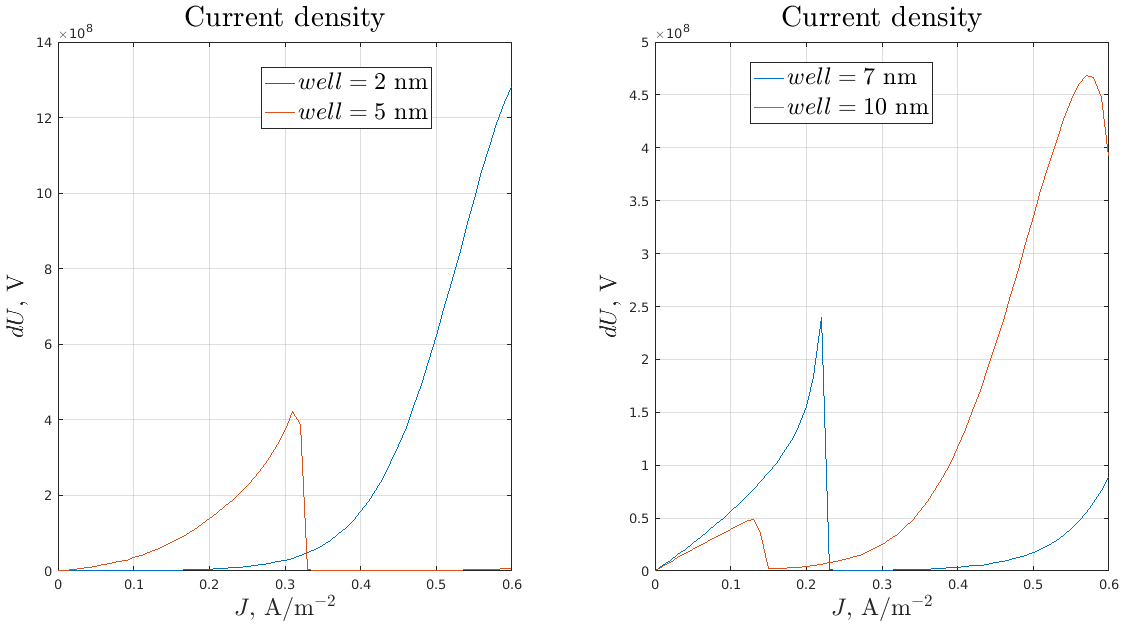
\includegraphics[width=0.9\linewidth]{qwwj.png}
	\caption{Плотность тока через РТГС при различных ширинах потенциальной ямы}
	\label{fig:qwwj}
\end{figure}

\subsection{Вывод}

Глубина ямы влияет на величину тока, причем пиковое напряжение изменяется не значительно. Значительное влияние на смещение пикового напряжения оказывает изменение ширины ПЯ.